\section{Knl\-Mat3d\_\-MPI Class Reference}
\label{classKnlMat3d__MPI}\index{KnlMat3d_MPI@{KnlMat3d\_\-MPI}}
{\tt \#include $<$knlmat3d\_\-mpi.hpp$>$}

Inheritance diagram for Knl\-Mat3d\_\-MPI::\begin{figure}[H]
\begin{center}
\leavevmode
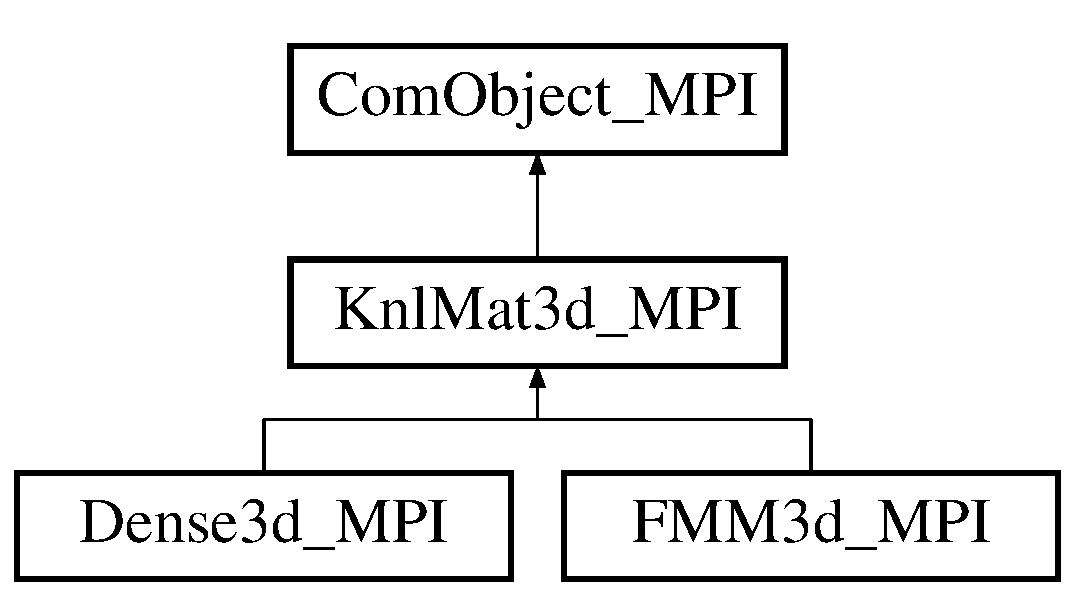
\includegraphics[height=3cm]{classKnlMat3d__MPI}
\end{center}
\end{figure}


\subsection{Detailed Description}
Knl\-Mat3d\_\-MPI is an mpi version of Knl\-Mat3d - storing kernel and matrix information for 3d. Knl\-Mat3d\_\-MPI builds upon {\bf Com\-Object\_\-MPI}{\rm (p.\,\pageref{classComObject__MPI})} - for use with FMM\_\-3d\_\-MPI or {\bf Dense3d\_\-MPI}{\rm (p.\,\pageref{classDense3d__MPI})} by including virtual functions for {\bf setup()}{\rm (p.\,\pageref{classKnlMat3d__MPI_98f7aa1beebfd344710d076d3d6413a2_98f7aa1beebfd344710d076d3d6413a2})} and evaluate(...) as well as accesses to information such as source positions, target values, etc. 



Definition at line 29 of file knlmat3d\_\-mpi.hpp.\subsection*{Public Member Functions}
\begin{CompactItemize}
\item 
{\bf Knl\-Mat3d\_\-MPI} (const string \&p)
\item 
virtual {\bf $\sim$Knl\-Mat3d\_\-MPI} ()
\item 
Vec \& {\bf src\-Pos} ()
\item 
Vec \& {\bf src\-Nor} ()
\item 
Vec \& {\bf trg\-Pos} ()
\item 
{\bf Kernel3d\_\-MPI} \& {\bf knl} ()
\item 
virtual int {\bf setup} ()=0
\item 
virtual int {\bf evaluate} (Vec src\-Den, Vec trg\-Val)=0
\item 
int {\bf dim} ()
\item 
int {\bf src\-DOF} ()
\item 
int {\bf trg\-DOF} ()
\item 
int {\bf proc\-Lcl\-Num} (Vec pos)
\item 
int {\bf proc\-Glb\-Num} (Vec pos)
\item 
void {\bf proc\-Lcl\-Ran} (Vec pos, int \&beg, int \&end)
\end{CompactItemize}
\subsection*{Protected Attributes}
\begin{CompactItemize}
\item 
Vec {\bf \_\-src\-Pos}
\item 
Vec {\bf \_\-src\-Nor}
\item 
Vec {\bf \_\-trg\-Pos}
\item 
{\bf Kernel3d\_\-MPI} {\bf \_\-knl}
\end{CompactItemize}


\subsection{Constructor \& Destructor Documentation}
\index{KnlMat3d_MPI@{Knl\-Mat3d\_\-MPI}!KnlMat3d_MPI@{KnlMat3d\_\-MPI}}
\index{KnlMat3d_MPI@{KnlMat3d\_\-MPI}!KnlMat3d_MPI@{Knl\-Mat3d\_\-MPI}}
\subsubsection{\setlength{\rightskip}{0pt plus 5cm}Knl\-Mat3d\_\-MPI::Knl\-Mat3d\_\-MPI (const string \& {\em p})\hspace{0.3cm}{\tt  [inline]}}\label{classKnlMat3d__MPI_c66fe250a6e3b06ad193f069d8153419_c66fe250a6e3b06ad193f069d8153419}


Construct the Knl\-Mat3d\_\-MPI object, using a string, which is passed to Com\-Object. For example, \char`\"{}fmm3d\_\-\char`\"{} for fmm3d. \_\-src\-Pos, \_\-src\-Nor, and \_\-trg\-Pos are set to NULL 

Definition at line 44 of file knlmat3d\_\-mpi.hpp.

\footnotesize\begin{verbatim}44                                : 
45          ComObject_MPI(p), _srcPos(NULL), _srcNor(NULL), _trgPos(NULL) {;}
\end{verbatim}\normalsize 


\index{KnlMat3d_MPI@{Knl\-Mat3d\_\-MPI}!~KnlMat3d_MPI@{$\sim$KnlMat3d\_\-MPI}}
\index{~KnlMat3d_MPI@{$\sim$KnlMat3d\_\-MPI}!KnlMat3d_MPI@{Knl\-Mat3d\_\-MPI}}
\subsubsection{\setlength{\rightskip}{0pt plus 5cm}virtual Knl\-Mat3d\_\-MPI::$\sim$Knl\-Mat3d\_\-MPI ()\hspace{0.3cm}{\tt  [inline, virtual]}}\label{classKnlMat3d__MPI_79335cbcac8d5b9babe0b4a6394e2caa_79335cbcac8d5b9babe0b4a6394e2caa}


destructor - calls $\sim$Com\-Object() 

Definition at line 47 of file knlmat3d\_\-mpi.hpp.

\footnotesize\begin{verbatim}47 { }
\end{verbatim}\normalsize 




\subsection{Member Function Documentation}
\index{KnlMat3d_MPI@{Knl\-Mat3d\_\-MPI}!dim@{dim}}
\index{dim@{dim}!KnlMat3d_MPI@{Knl\-Mat3d\_\-MPI}}
\subsubsection{\setlength{\rightskip}{0pt plus 5cm}int Knl\-Mat3d\_\-MPI::dim ()\hspace{0.3cm}{\tt  [inline]}}\label{classKnlMat3d__MPI_e3f9953141ca7d7525b58c0ff1ef6b1f_e3f9953141ca7d7525b58c0ff1ef6b1f}


Return dimension of the problem. Set to 3 

Definition at line 65 of file knlmat3d\_\-mpi.hpp.

Referenced by FMM3d\_\-MPI::check(), FMM3d\_\-MPI::ctb\-Src\-Exa\-Nor(), Dense3d\_\-MPI::evaluate(), FMM3d\_\-MPI::eva\-Trg\-Exa\-Pos(), proc\-Glb\-Num(), proc\-Lcl\-Num(), proc\-Lcl\-Ran(), FMM3d\_\-MPI::usr\-Src\-Exa\-Nor(), and FMM3d\_\-MPI::usr\-Src\-Exa\-Pos().

\footnotesize\begin{verbatim}65 { return 3; }
\end{verbatim}\normalsize 


\index{KnlMat3d_MPI@{Knl\-Mat3d\_\-MPI}!evaluate@{evaluate}}
\index{evaluate@{evaluate}!KnlMat3d_MPI@{Knl\-Mat3d\_\-MPI}}
\subsubsection{\setlength{\rightskip}{0pt plus 5cm}virtual int Knl\-Mat3d\_\-MPI::evaluate (Vec {\em src\-Den}, Vec {\em trg\-Val})\hspace{0.3cm}{\tt  [pure virtual]}}\label{classKnlMat3d__MPI_abf7f0a466fbc47db0804a35093c819f_abf7f0a466fbc47db0804a35093c819f}


virtual evaluation function. takes source densities and evaluates target values depending on kernel 

Implemented in {\bf Dense3d\_\-MPI} {\rm (p.\,\pageref{classDense3d__MPI_b6d6d5d529463497e5bed037a921cfc2_b6d6d5d529463497e5bed037a921cfc2})}, and {\bf FMM3d\_\-MPI} {\rm (p.\,\pageref{classFMM3d__MPI_8db45026f69e4b2b504f0c491c170d7d_8db45026f69e4b2b504f0c491c170d7d})}.\index{KnlMat3d_MPI@{Knl\-Mat3d\_\-MPI}!knl@{knl}}
\index{knl@{knl}!KnlMat3d_MPI@{Knl\-Mat3d\_\-MPI}}
\subsubsection{\setlength{\rightskip}{0pt plus 5cm}{\bf Kernel3d\_\-MPI}\& Knl\-Mat3d\_\-MPI::knl ()\hspace{0.3cm}{\tt  [inline]}}\label{classKnlMat3d__MPI_d01911fc223ab4bc9604db12f942194e_d01911fc223ab4bc9604db12f942194e}




Definition at line 56 of file knlmat3d\_\-mpi.hpp.

References \_\-knl.

Referenced by main().

\footnotesize\begin{verbatim}56 { return _knl; }
\end{verbatim}\normalsize 


\index{KnlMat3d_MPI@{Knl\-Mat3d\_\-MPI}!procGlbNum@{procGlbNum}}
\index{procGlbNum@{procGlbNum}!KnlMat3d_MPI@{Knl\-Mat3d\_\-MPI}}
\subsubsection{\setlength{\rightskip}{0pt plus 5cm}int Knl\-Mat3d\_\-MPI::proc\-Glb\-Num (Vec {\em pos})\hspace{0.3cm}{\tt  [inline]}}\label{classKnlMat3d__MPI_47cb2afea618c56a5cc6e05f4034a806_47cb2afea618c56a5cc6e05f4034a806}


global number of positions for this processor 

Definition at line 74 of file knlmat3d\_\-mpi.hpp.

References dim().

Referenced by FMM3d\_\-MPI::evaluate(), and Dense3d\_\-MPI::evaluate().

\footnotesize\begin{verbatim}74 { int tmp; VecGetSize(     pos, &tmp); return tmp/dim(); }
\end{verbatim}\normalsize 


\index{KnlMat3d_MPI@{Knl\-Mat3d\_\-MPI}!procLclNum@{procLclNum}}
\index{procLclNum@{procLclNum}!KnlMat3d_MPI@{Knl\-Mat3d\_\-MPI}}
\subsubsection{\setlength{\rightskip}{0pt plus 5cm}int Knl\-Mat3d\_\-MPI::proc\-Lcl\-Num (Vec {\em pos})\hspace{0.3cm}{\tt  [inline]}}\label{classKnlMat3d__MPI_21f80b863e1376ff6648d882fdabd08e_21f80b863e1376ff6648d882fdabd08e}


local number of positions for this processor 

Definition at line 72 of file knlmat3d\_\-mpi.hpp.

References dim().

Referenced by FMM3d\_\-MPI::check(), and Dense3d\_\-MPI::evaluate().

\footnotesize\begin{verbatim}72 { int tmp; VecGetLocalSize(pos, &tmp); return tmp/dim(); }
\end{verbatim}\normalsize 


\index{KnlMat3d_MPI@{Knl\-Mat3d\_\-MPI}!procLclRan@{procLclRan}}
\index{procLclRan@{procLclRan}!KnlMat3d_MPI@{Knl\-Mat3d\_\-MPI}}
\subsubsection{\setlength{\rightskip}{0pt plus 5cm}void Knl\-Mat3d\_\-MPI::proc\-Lcl\-Ran (Vec {\em pos}, int \& {\em beg}, int \& {\em end})\hspace{0.3cm}{\tt  [inline]}}\label{classKnlMat3d__MPI_c77ddf71aecd48cd8a8ed887d5bcd834_c77ddf71aecd48cd8a8ed887d5bcd834}


processor Local Range. for vector pos, return the beginning and end range positions for which the local processor is responsible 

Definition at line 77 of file knlmat3d\_\-mpi.hpp.

References dim().

\footnotesize\begin{verbatim}77 { VecGetOwnershipRange(pos, &beg, &end); beg=beg/dim(); end=end/dim(); }
\end{verbatim}\normalsize 


\index{KnlMat3d_MPI@{Knl\-Mat3d\_\-MPI}!setup@{setup}}
\index{setup@{setup}!KnlMat3d_MPI@{Knl\-Mat3d\_\-MPI}}
\subsubsection{\setlength{\rightskip}{0pt plus 5cm}virtual int Knl\-Mat3d\_\-MPI::setup ()\hspace{0.3cm}{\tt  [pure virtual]}}\label{classKnlMat3d__MPI_98f7aa1beebfd344710d076d3d6413a2_98f7aa1beebfd344710d076d3d6413a2}


virtual setup function 

Implemented in {\bf Dense3d\_\-MPI} {\rm (p.\,\pageref{classDense3d__MPI_415266b005d267e801176f27c0434a50_415266b005d267e801176f27c0434a50})}, and {\bf FMM3d\_\-MPI} {\rm (p.\,\pageref{classFMM3d__MPI_415266b005d267e801176f27c0434a50_415266b005d267e801176f27c0434a50})}.\index{KnlMat3d_MPI@{Knl\-Mat3d\_\-MPI}!srcDOF@{srcDOF}}
\index{srcDOF@{srcDOF}!KnlMat3d_MPI@{Knl\-Mat3d\_\-MPI}}
\subsubsection{\setlength{\rightskip}{0pt plus 5cm}int Knl\-Mat3d\_\-MPI::src\-DOF ()\hspace{0.3cm}{\tt  [inline]}}\label{classKnlMat3d__MPI_6b422ba557bb24eff82ac7125e206568_6b422ba557bb24eff82ac7125e206568}


Return source degree of freedom: \_\-knl.src\-DOF() - see {\bf kernel3d\_\-mpi.hpp}{\rm (p.\,\pageref{kernel3d__mpi_8hpp})} 

Definition at line 67 of file knlmat3d\_\-mpi.hpp.

References \_\-knl, and Kernel3d\_\-MPI::src\-DOF().

Referenced by FMM3d\_\-MPI::check(), FMM3d\_\-MPI::ctb\-Src\-Exa\-Den(), FMM3d\_\-MPI::evaluate(), Dense3d\_\-MPI::evaluate(), and FMM3d\_\-MPI::usr\-Src\-Exa\-Den().

\footnotesize\begin{verbatim}67 { return _knl.srcDOF(); }
\end{verbatim}\normalsize 


\index{KnlMat3d_MPI@{Knl\-Mat3d\_\-MPI}!srcNor@{srcNor}}
\index{srcNor@{srcNor}!KnlMat3d_MPI@{Knl\-Mat3d\_\-MPI}}
\subsubsection{\setlength{\rightskip}{0pt plus 5cm}Vec\& Knl\-Mat3d\_\-MPI::src\-Nor ()\hspace{0.3cm}{\tt  [inline]}}\label{classKnlMat3d__MPI_bba2c6a917421951f1fbe8f69b9a135b_bba2c6a917421951f1fbe8f69b9a135b}


Return source normals 

Definition at line 52 of file knlmat3d\_\-mpi.hpp.

References \_\-src\-Nor.

Referenced by main().

\footnotesize\begin{verbatim}52 { return _srcNor; }
\end{verbatim}\normalsize 


\index{KnlMat3d_MPI@{Knl\-Mat3d\_\-MPI}!srcPos@{srcPos}}
\index{srcPos@{srcPos}!KnlMat3d_MPI@{Knl\-Mat3d\_\-MPI}}
\subsubsection{\setlength{\rightskip}{0pt plus 5cm}Vec\& Knl\-Mat3d\_\-MPI::src\-Pos ()\hspace{0.3cm}{\tt  [inline]}}\label{classKnlMat3d__MPI_caa1dae06f56964efa0f778b696dce61_caa1dae06f56964efa0f778b696dce61}


Return source positions 

Definition at line 50 of file knlmat3d\_\-mpi.hpp.

References \_\-src\-Pos.

Referenced by main().

\footnotesize\begin{verbatim}50 { return _srcPos; }
\end{verbatim}\normalsize 


\index{KnlMat3d_MPI@{Knl\-Mat3d\_\-MPI}!trgDOF@{trgDOF}}
\index{trgDOF@{trgDOF}!KnlMat3d_MPI@{Knl\-Mat3d\_\-MPI}}
\subsubsection{\setlength{\rightskip}{0pt plus 5cm}int Knl\-Mat3d\_\-MPI::trg\-DOF ()\hspace{0.3cm}{\tt  [inline]}}\label{classKnlMat3d__MPI_ea43c1f768349e86110e4e2d06e38d10_ea43c1f768349e86110e4e2d06e38d10}


Return target degree of freedom: \_\-knl.trg\-DOF() - see {\bf kernel3d\_\-mpi.hpp}{\rm (p.\,\pageref{kernel3d__mpi_8hpp})} 

Definition at line 69 of file knlmat3d\_\-mpi.hpp.

References \_\-knl, and Kernel3d\_\-MPI::trg\-DOF().

Referenced by FMM3d\_\-MPI::check(), FMM3d\_\-MPI::evaluate(), Dense3d\_\-MPI::evaluate(), and FMM3d\_\-MPI::eva\-Trg\-Exa\-Val().

\footnotesize\begin{verbatim}69 { return _knl.trgDOF(); }
\end{verbatim}\normalsize 


\index{KnlMat3d_MPI@{Knl\-Mat3d\_\-MPI}!trgPos@{trgPos}}
\index{trgPos@{trgPos}!KnlMat3d_MPI@{Knl\-Mat3d\_\-MPI}}
\subsubsection{\setlength{\rightskip}{0pt plus 5cm}Vec\& Knl\-Mat3d\_\-MPI::trg\-Pos ()\hspace{0.3cm}{\tt  [inline]}}\label{classKnlMat3d__MPI_7dc770563c182703b1986abb06c6dbbd_7dc770563c182703b1986abb06c6dbbd}


Return target positions 

Definition at line 54 of file knlmat3d\_\-mpi.hpp.

References \_\-trg\-Pos.

Referenced by main().

\footnotesize\begin{verbatim}54 { return _trgPos; }
\end{verbatim}\normalsize 




\subsection{Member Data Documentation}
\index{KnlMat3d_MPI@{Knl\-Mat3d\_\-MPI}!_knl@{\_\-knl}}
\index{_knl@{\_\-knl}!KnlMat3d_MPI@{Knl\-Mat3d\_\-MPI}}
\subsubsection{\setlength{\rightskip}{0pt plus 5cm}{\bf Kernel3d\_\-MPI} {\bf Knl\-Mat3d\_\-MPI::\_\-knl}\hspace{0.3cm}{\tt  [protected]}}\label{classKnlMat3d__MPI_cb56a4f532a89bc1a51ee17c2434a106_cb56a4f532a89bc1a51ee17c2434a106}


the kernel being used, defined in {\bf kernel3d\_\-mpi.hpp}{\rm (p.\,\pageref{kernel3d__mpi_8hpp})} - defines kernel type and coefficients 

Definition at line 40 of file knlmat3d\_\-mpi.hpp.

Referenced by Dense3d\_\-MPI::evaluate(), knl(), FMM3d\_\-MPI::setup(), src\-DOF(), FMM3d\_\-MPI::Src\-Equ2Trg\-Chk\_\-dgemv(), and trg\-DOF().\index{KnlMat3d_MPI@{Knl\-Mat3d\_\-MPI}!_srcNor@{\_\-srcNor}}
\index{_srcNor@{\_\-srcNor}!KnlMat3d_MPI@{Knl\-Mat3d\_\-MPI}}
\subsubsection{\setlength{\rightskip}{0pt plus 5cm}Vec {\bf Knl\-Mat3d\_\-MPI::\_\-src\-Nor}\hspace{0.3cm}{\tt  [protected]}}\label{classKnlMat3d__MPI_bbeec6db21041e1b277f4755f21047dd_bbeec6db21041e1b277f4755f21047dd}


Source normals 

Definition at line 36 of file knlmat3d\_\-mpi.hpp.

Referenced by Dense3d\_\-MPI::evaluate(), FMM3d\_\-MPI::setup(), Dense3d\_\-MPI::setup(), and src\-Nor().\index{KnlMat3d_MPI@{Knl\-Mat3d\_\-MPI}!_srcPos@{\_\-srcPos}}
\index{_srcPos@{\_\-srcPos}!KnlMat3d_MPI@{Knl\-Mat3d\_\-MPI}}
\subsubsection{\setlength{\rightskip}{0pt plus 5cm}Vec {\bf Knl\-Mat3d\_\-MPI::\_\-src\-Pos}\hspace{0.3cm}{\tt  [protected]}}\label{classKnlMat3d__MPI_f66b814fdf8eb17df56ff5ff27a368da_f66b814fdf8eb17df56ff5ff27a368da}


Source positions 

Definition at line 34 of file knlmat3d\_\-mpi.hpp.

Referenced by FMM3d\_\-MPI::check(), FMM3d\_\-MPI::evaluate(), Dense3d\_\-MPI::evaluate(), FMM3d\_\-MPI::setup(), Dense3d\_\-MPI::setup(), and src\-Pos().\index{KnlMat3d_MPI@{Knl\-Mat3d\_\-MPI}!_trgPos@{\_\-trgPos}}
\index{_trgPos@{\_\-trgPos}!KnlMat3d_MPI@{Knl\-Mat3d\_\-MPI}}
\subsubsection{\setlength{\rightskip}{0pt plus 5cm}Vec {\bf Knl\-Mat3d\_\-MPI::\_\-trg\-Pos}\hspace{0.3cm}{\tt  [protected]}}\label{classKnlMat3d__MPI_a1b44c7c6fd0a38be167c34537b1a508_a1b44c7c6fd0a38be167c34537b1a508}


Target positions 

Definition at line 38 of file knlmat3d\_\-mpi.hpp.

Referenced by FMM3d\_\-MPI::check(), FMM3d\_\-MPI::evaluate(), Dense3d\_\-MPI::evaluate(), FMM3d\_\-MPI::setup(), Dense3d\_\-MPI::setup(), and trg\-Pos().

The documentation for this class was generated from the following file:\begin{CompactItemize}
\item 
fmm3d\_\-mpi/{\bf knlmat3d\_\-mpi.hpp}\end{CompactItemize}
